Každý model je složen ze tří základních složek a to \uv{vertices}, \uv{edges} a \uv{faces}, které definují celkový tvar a vzhled. Pro tvorbu modelů do hry je využit \uv{Low Poly}\cite{LowPoly} styl, díky čemuž mají výsledné objekty menší počet polygonů a jsou více optimalizované. Pro tvorbu objektů byl využit software Blender, který je ideální volbou pro tvorbu 3D grafických podkladů pro hru. Herní modely jsou využity v Unity a mobilní aplikaci.

\subsection{Box modeling}
\uv{Box modeling}\cite{BoxModeling} je technika modelování, při které jsou využity pouze základní objekty (jako je krychle, koule, atd.). Tento objekt je následně použit k dosažení finálního tvaru objektu dle připraveného návrhu. Celkový cyklus je opakován s každým novým prvkem a jednotlivé modely jsou poté kombinovány k dosažení cílového tvaru.

\subsection{Low poly}
Pro tvorbu jednotlivých herních modelů je využit styl \uv{Low poly}\cite{LowPoly}, který nabízí vysokou optimalizaci pro herní využití. \uv{Low poly} modely vypadají jednoduché, přičemž představují zákaldní tvar představované věci.

\subsection{Jednotlové herní modely}
Na začátku tvoření modelů bylo hlavní vybrat dobu, či místo, do které hru zasadit. Herní modely jsou vymodelovány ve vytvořeném příběhu o magickém světě a kouzelníkovi zachraňujícím svoji planetu.

\subsubsection{Postavy}
\subsubsubsection{Hlavní postava}
Model hlavní postavy je klíčový, protože představuje hráče a jeho postup hrou doprovází na každém kroku. Jak můžeme vidět na obr. \ref{fig:hlavni-postava}, tak model kouzelníka je hravý a jednoduchý. K modelu je vytvořena také sada animací pro jednotlivé pohybové operace ve hře.

\begin{figure}[h]
    \centering
    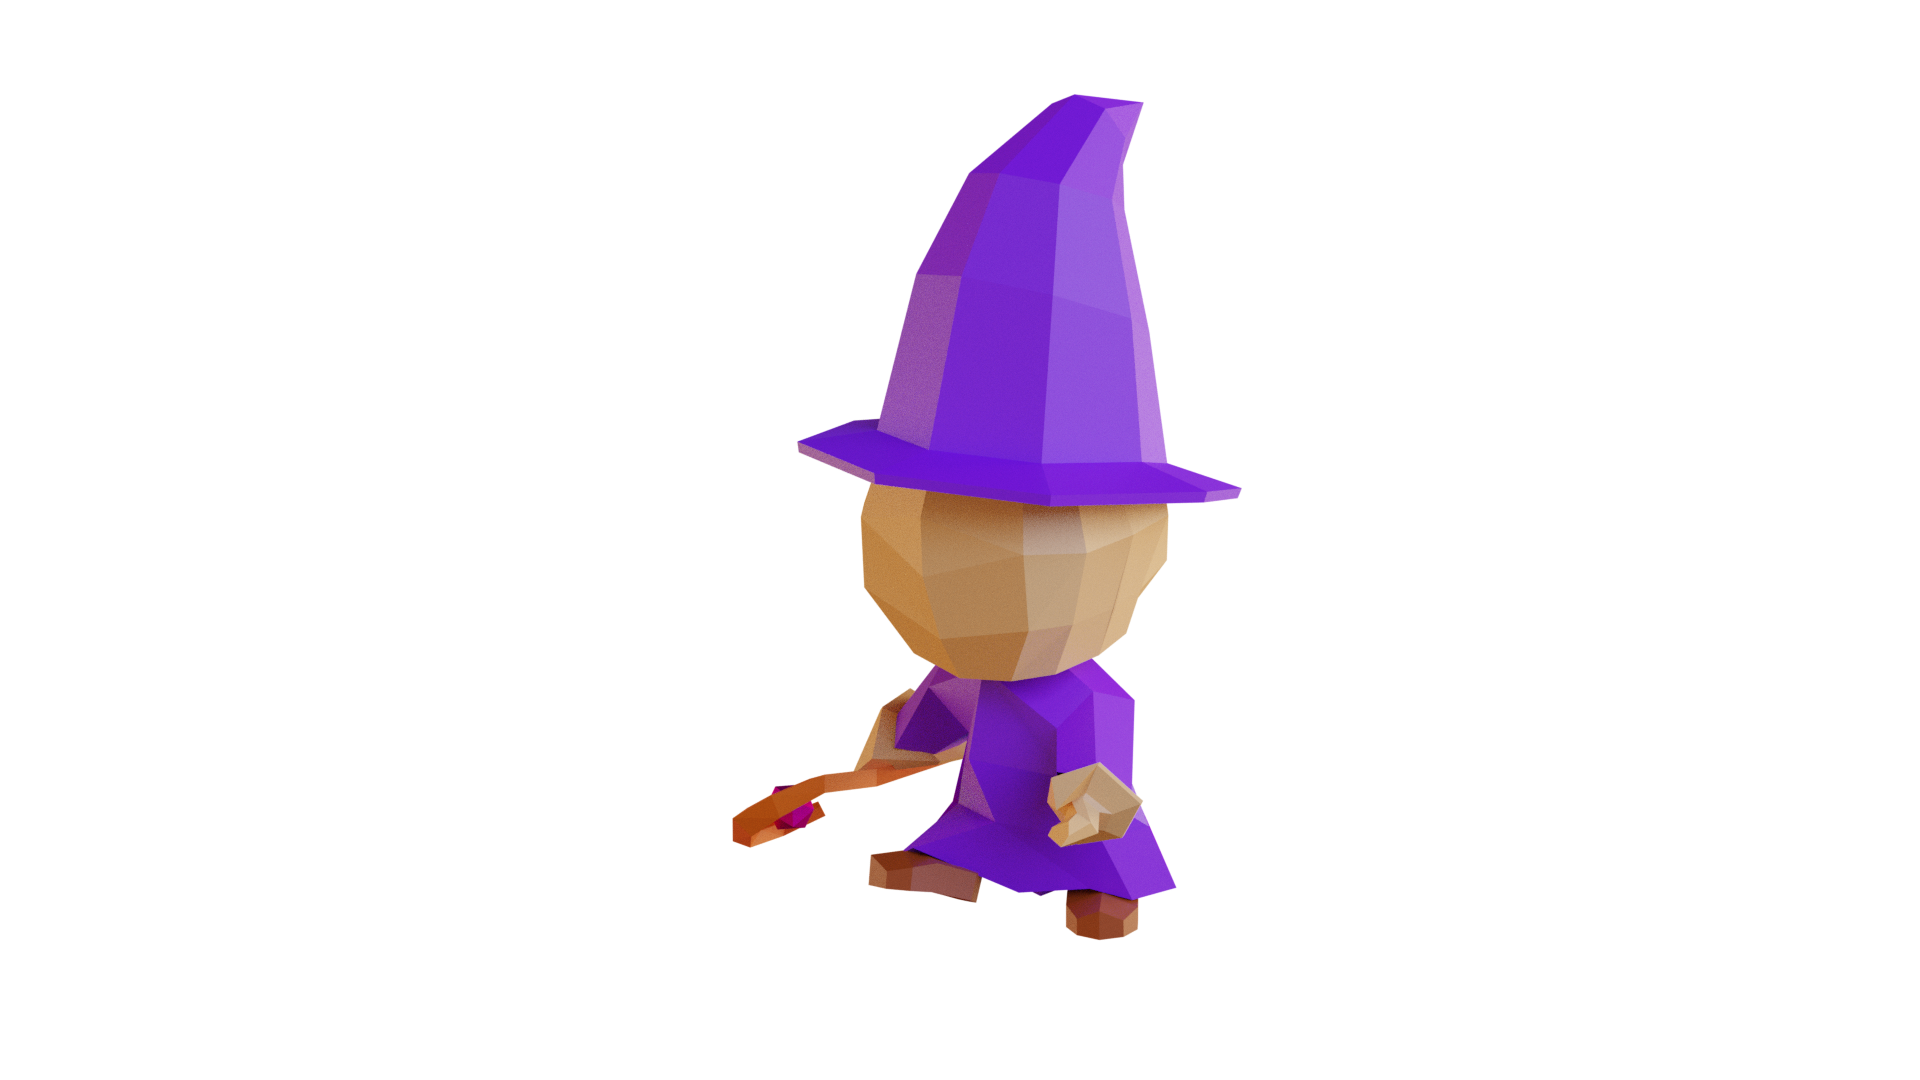
\includegraphics[width=0.6\textwidth]{img/hlavni-postava.png}
    \caption{Model hlavní postavy.}
    \label{fig:hlavni-postava}
\end{figure}

\subsubsubsection{Nepřátelé}
Každý ostrov má sadu nepřátel, které hráč může nalézt v jednotlivých úrovních. Nepřátelé mají za úkol hráči ztížit průchod úrovní. Jednotlivé nepřátelské jednotky mají sadu animací. Modely nepřátel můžeme vidět na obr. \ref{fig:nepritel-golem}, nebo obr. \ref{fig:nepritel-cerv}.

\begin{figure}[h]
    \centering
    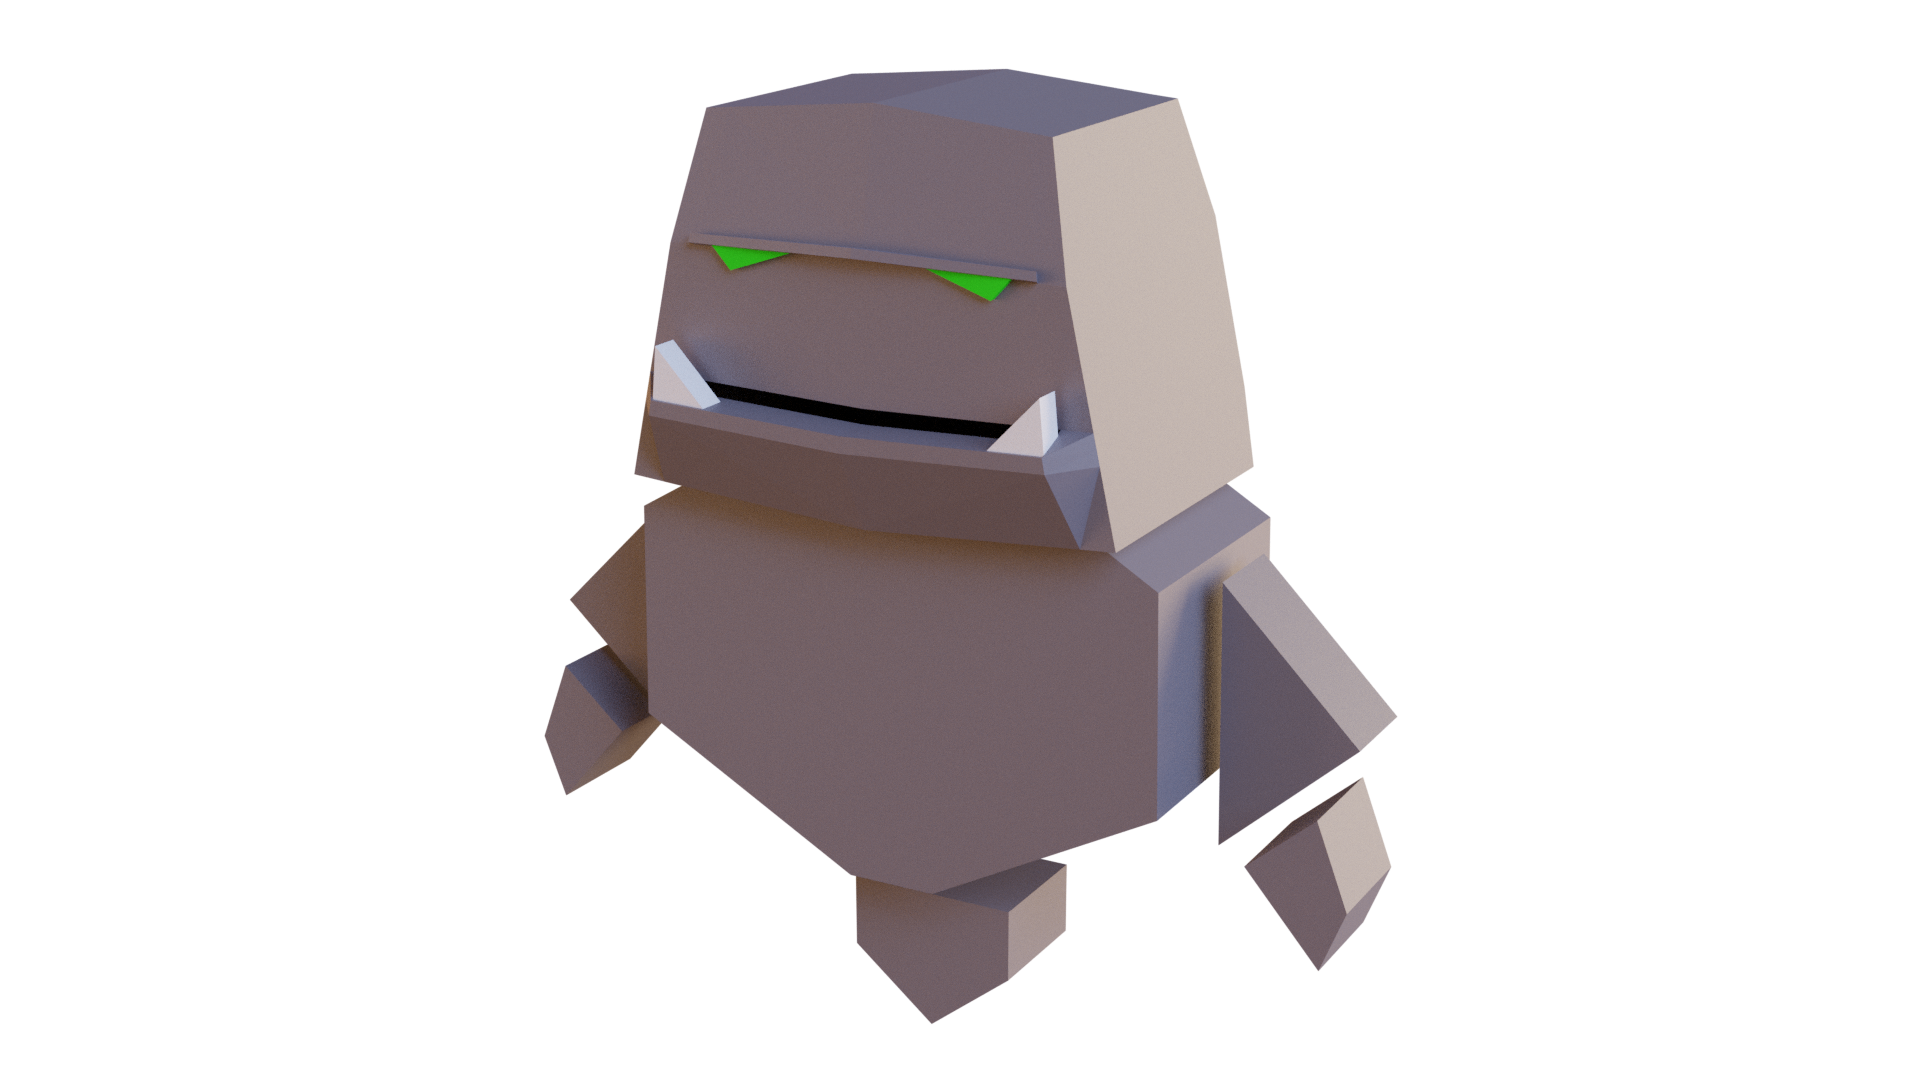
\includegraphics[width=0.6\textwidth]{img/nepritel-golem.png}
    \caption{Model nepřítele - Golem.}
    \label{fig:nepritel-golem}
\end{figure}

\begin{figure}[h]
    \centering
    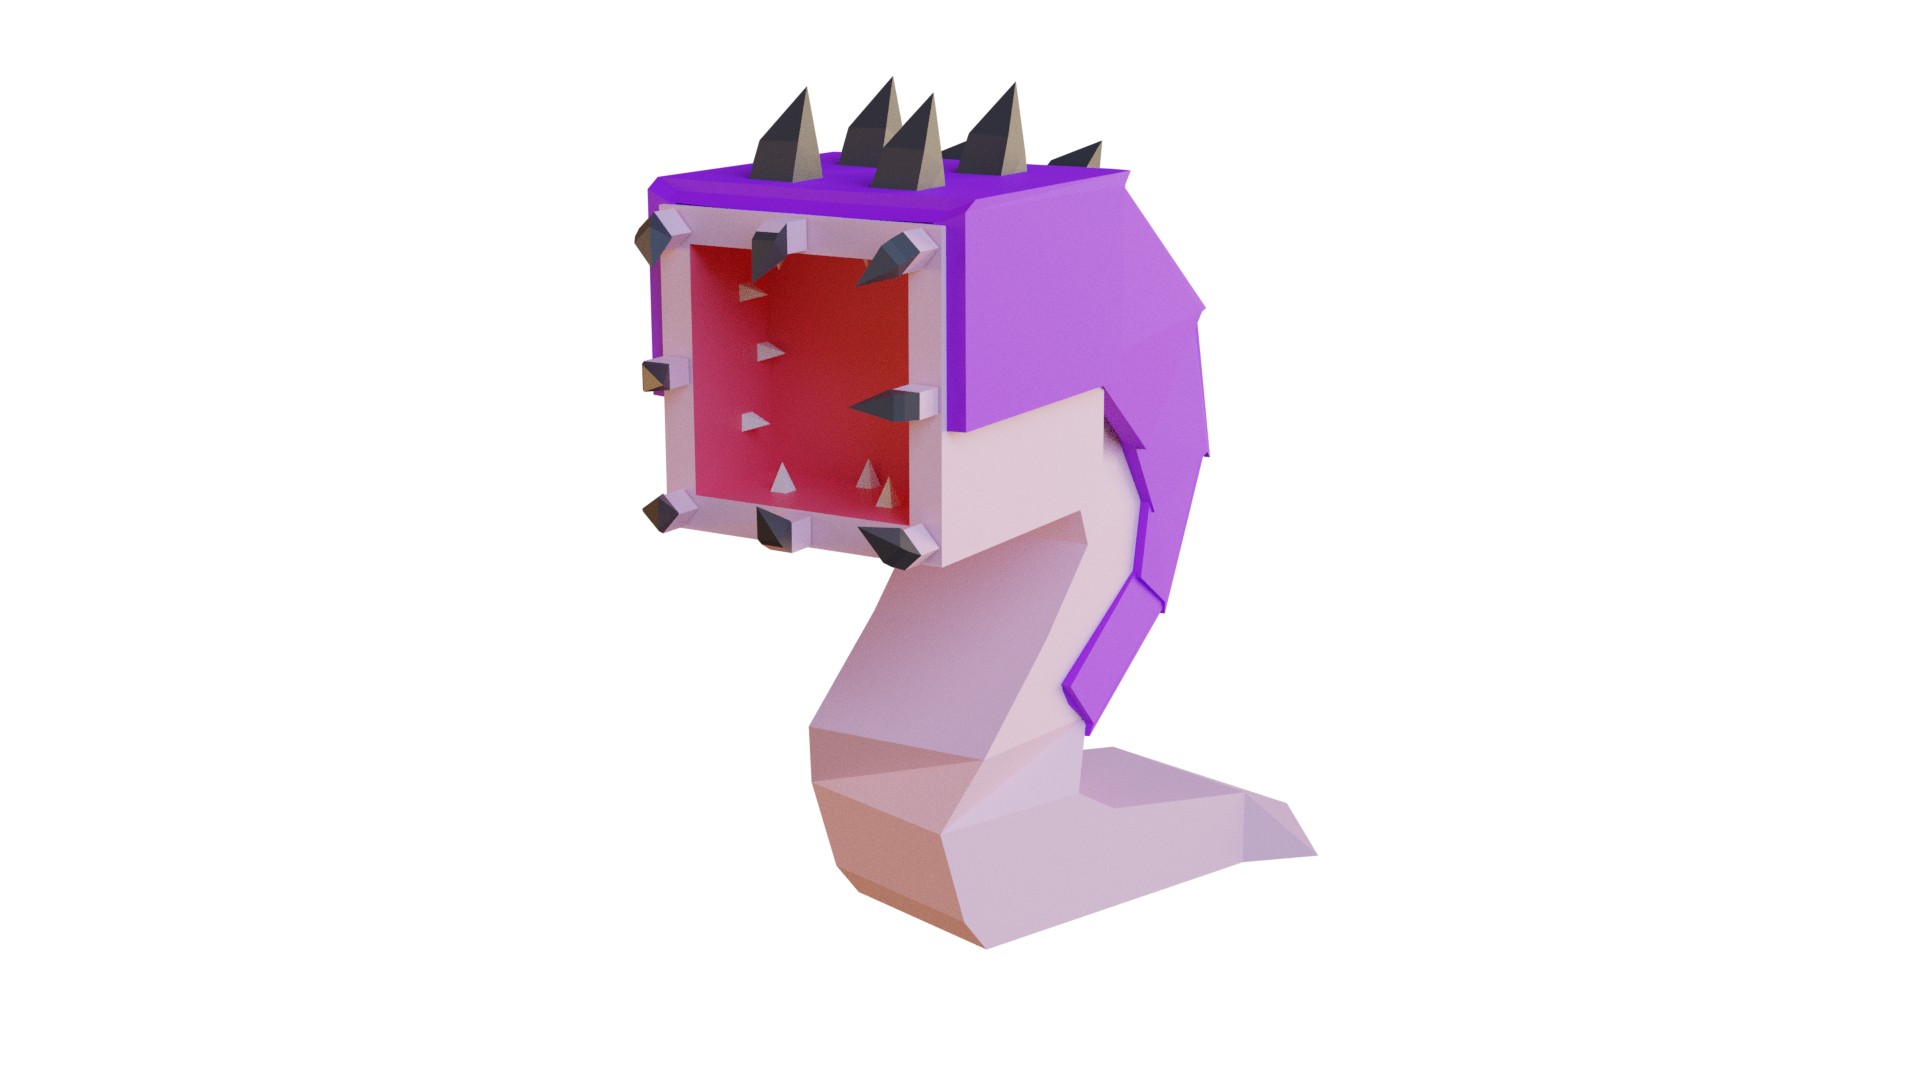
\includegraphics[width=0.6\textwidth]{img/nepritel-cerv.png}
    \caption{Model nepřítele - Červ.}
    \label{fig:nepritel-cerv}
\end{figure}

\subsubsection{Ostrovy}
Jednotlivé modely ostrovů představují přírodní elementy. Dle jednotlivých elementů jsou zbarvené a doplněné o modely, které jsou ve spojitosti s tímto elementem vyzobrazeny. Modely ostrovů jsou využity v mobilni aplikaci, jako je vidět na obr. \ref{fig:mobilni-aplikace-ostrov} Dominantou každého ostrova je krystal, který musí hráč získat pro úspěšné splnění. Ukázka zmiňovaných modelů obr. \ref{fig:nature-island}, obr. \ref{fig:fire-island} a obr. \ref{fig:winter-island}.

\begin{figure}[h]
    \centering
    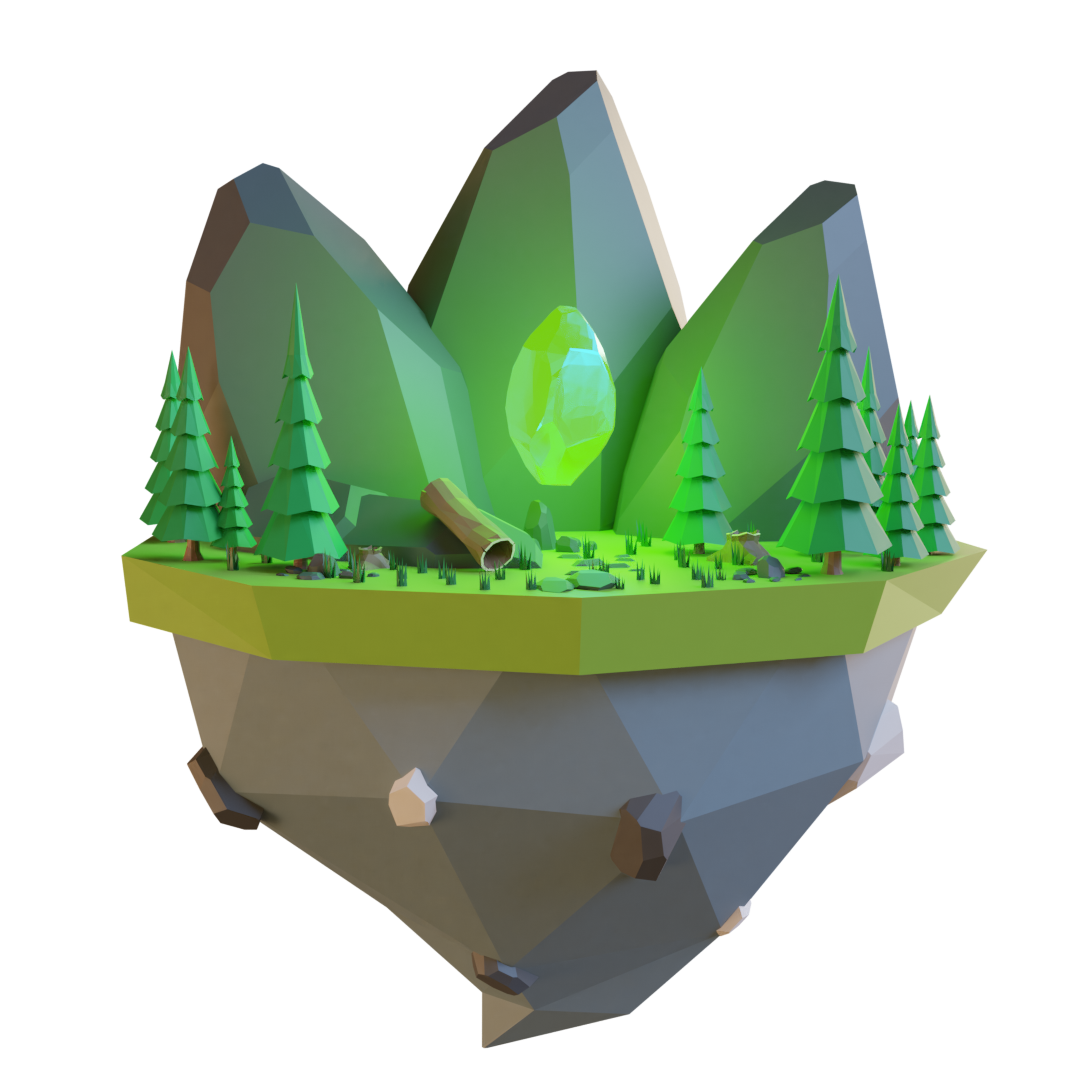
\includegraphics[width=0.6\textwidth]{img/NatureIsland.png}
    \caption{Model ostrova - Zemní ostrov.}
    \label{fig:nature-island}
\end{figure}

\begin{figure}[h]
    \centering
    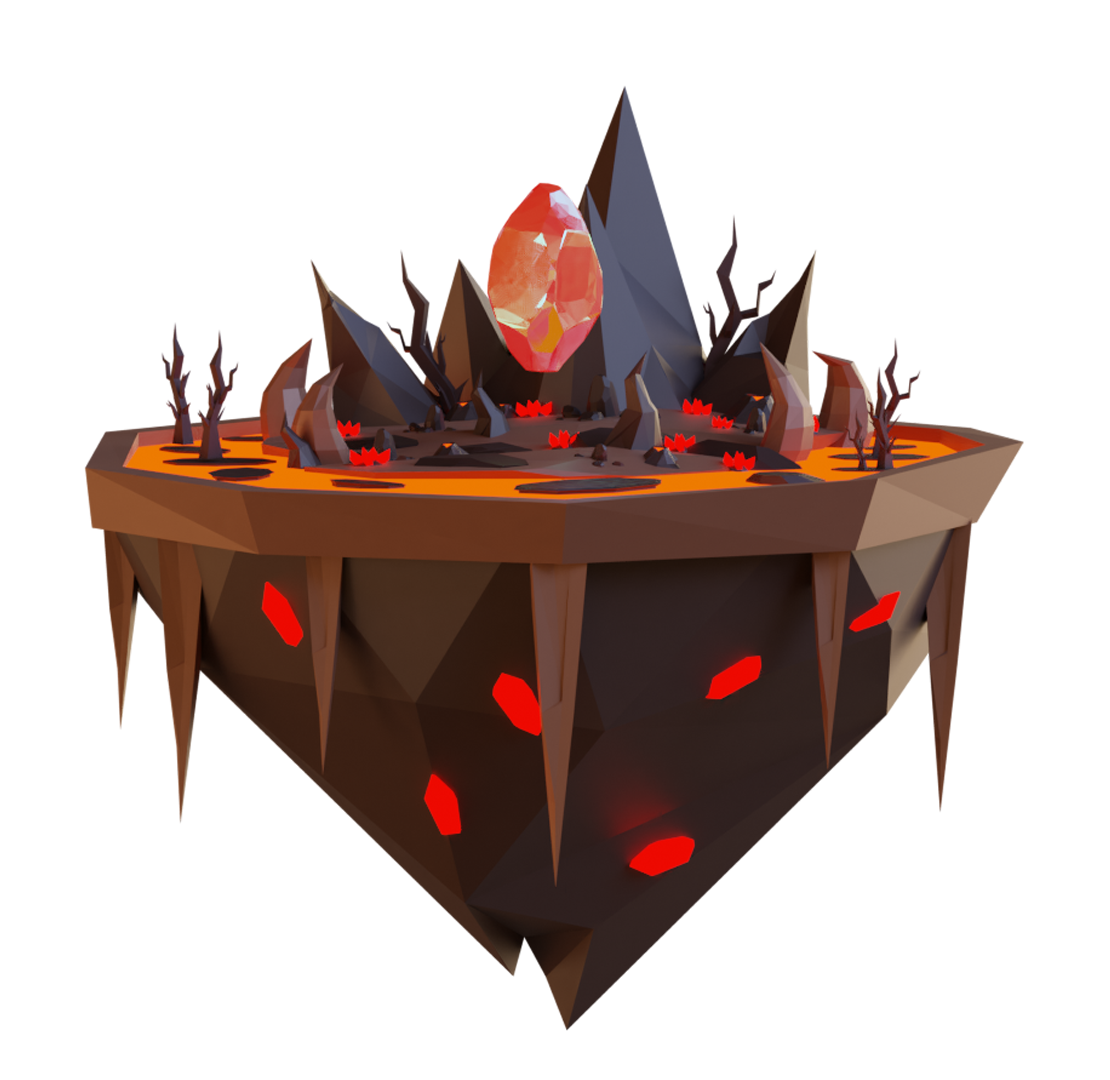
\includegraphics[width=0.6\textwidth]{img/FireIsland.png}
    \caption{Model ostrova - Ohnivý ostrov.}
    \label{fig:fire-island}
\end{figure}

\begin{figure}[h]
    \centering
    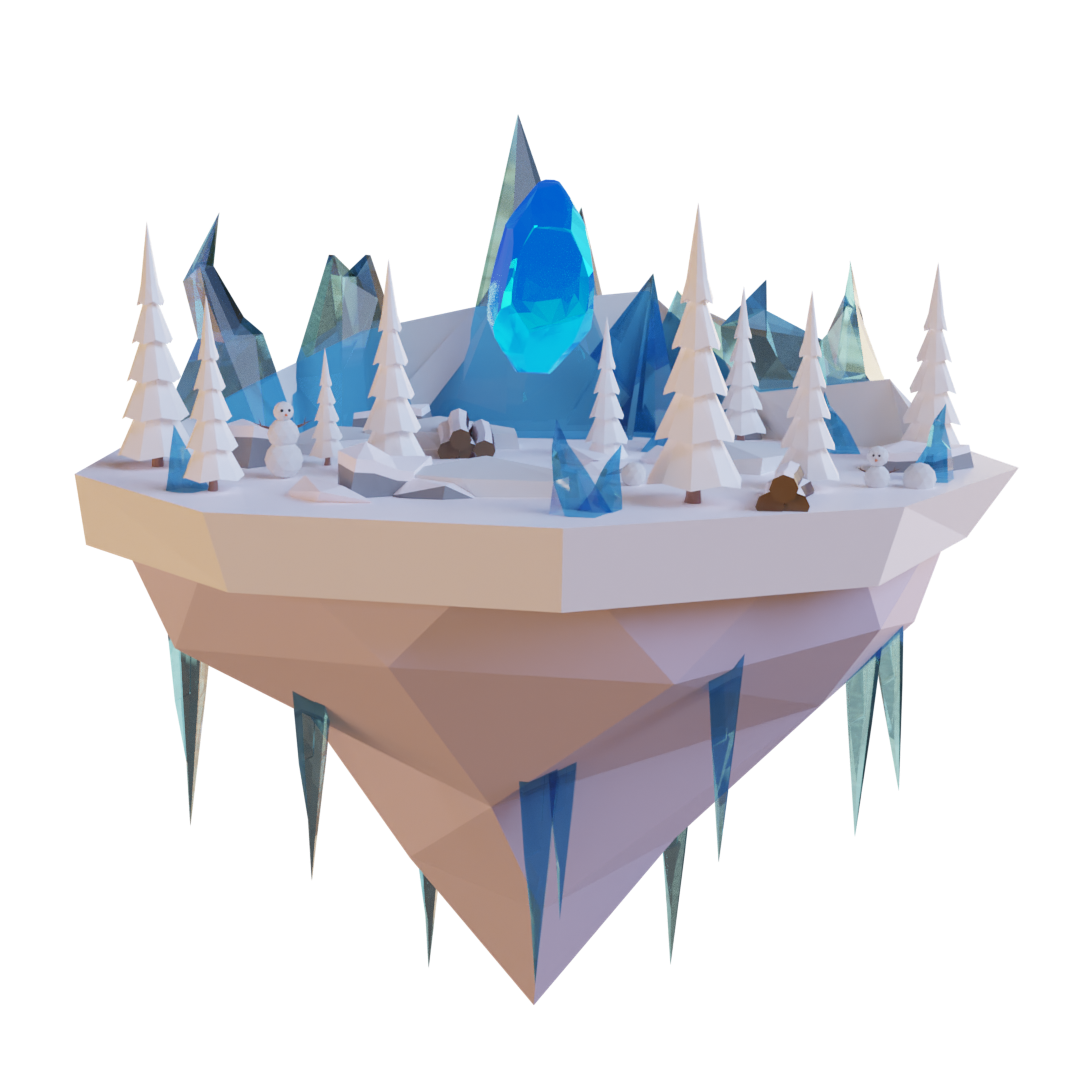
\includegraphics[width=0.6\textwidth]{img/WinterIsland.png}
    \caption{Model ostrova - Zimní ostrov.}
    \label{fig:winter-island}
\end{figure}

\begin{figure}[h]
    \centering
    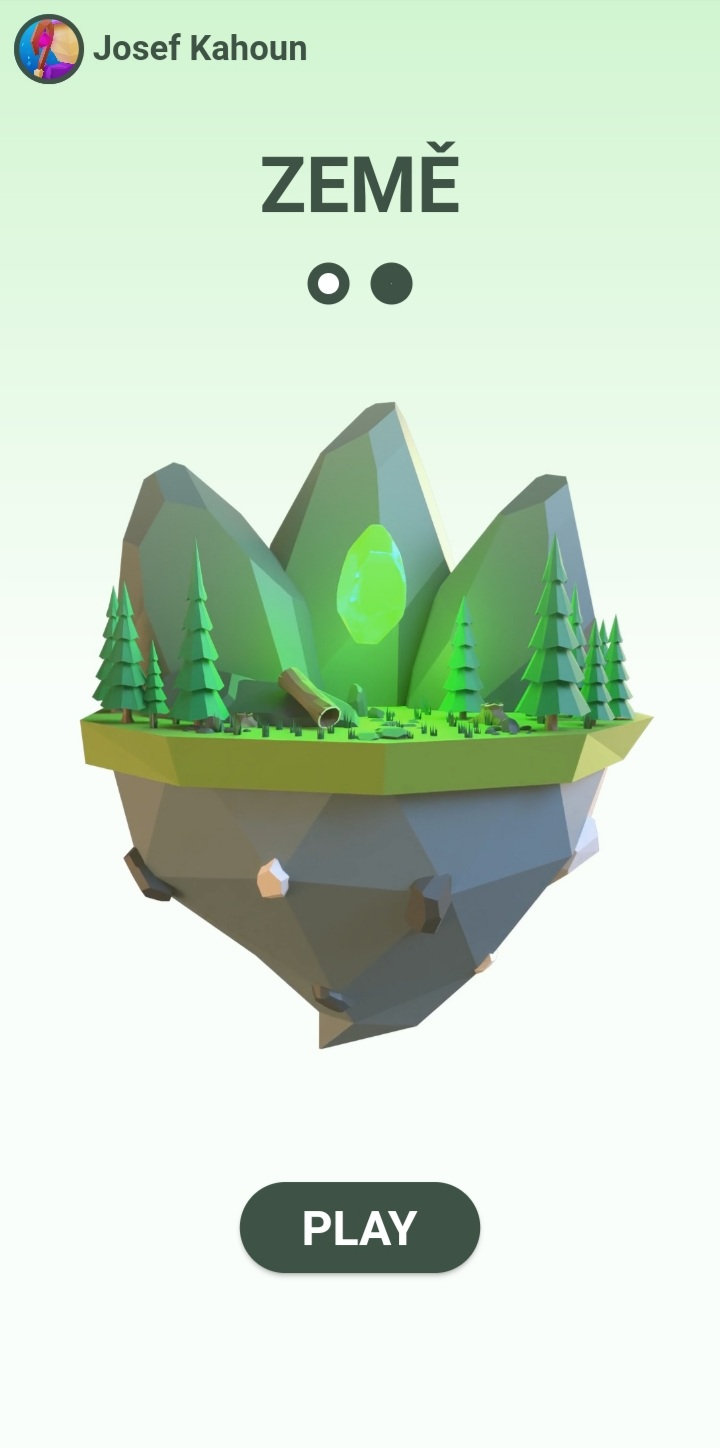
\includegraphics[width=0.6\textwidth]{img/mobilni-aplikace-ostrov.jpg}
    \caption{Model ostrova v mobilní aplikace.}
    \label{fig:mobilni-aplikace-ostrov}
\end{figure}

\subsubsubsection{Úrovně}
Jednotlivé úrovně tvoří mřížku, jako je vidět na obr. \ref{fig:model-levelu}. Úrovně představují stejný element, jako je ostrov, ke kterému patří. Celá hra je odehrávána na herních plošinách. Jednotlivé pole úrovně slouží jako umístitel herních postav, bariér, cest, či ukazatelů cíle. Prostředí okolo herních plošin je doplněno o modely mateřského ostrova. Úkázka herního prostředí jednotlivé úrovně, které můžete vidět na obr. \ref{fig:model-levelu}

\begin{figure}[h]
    \centering
    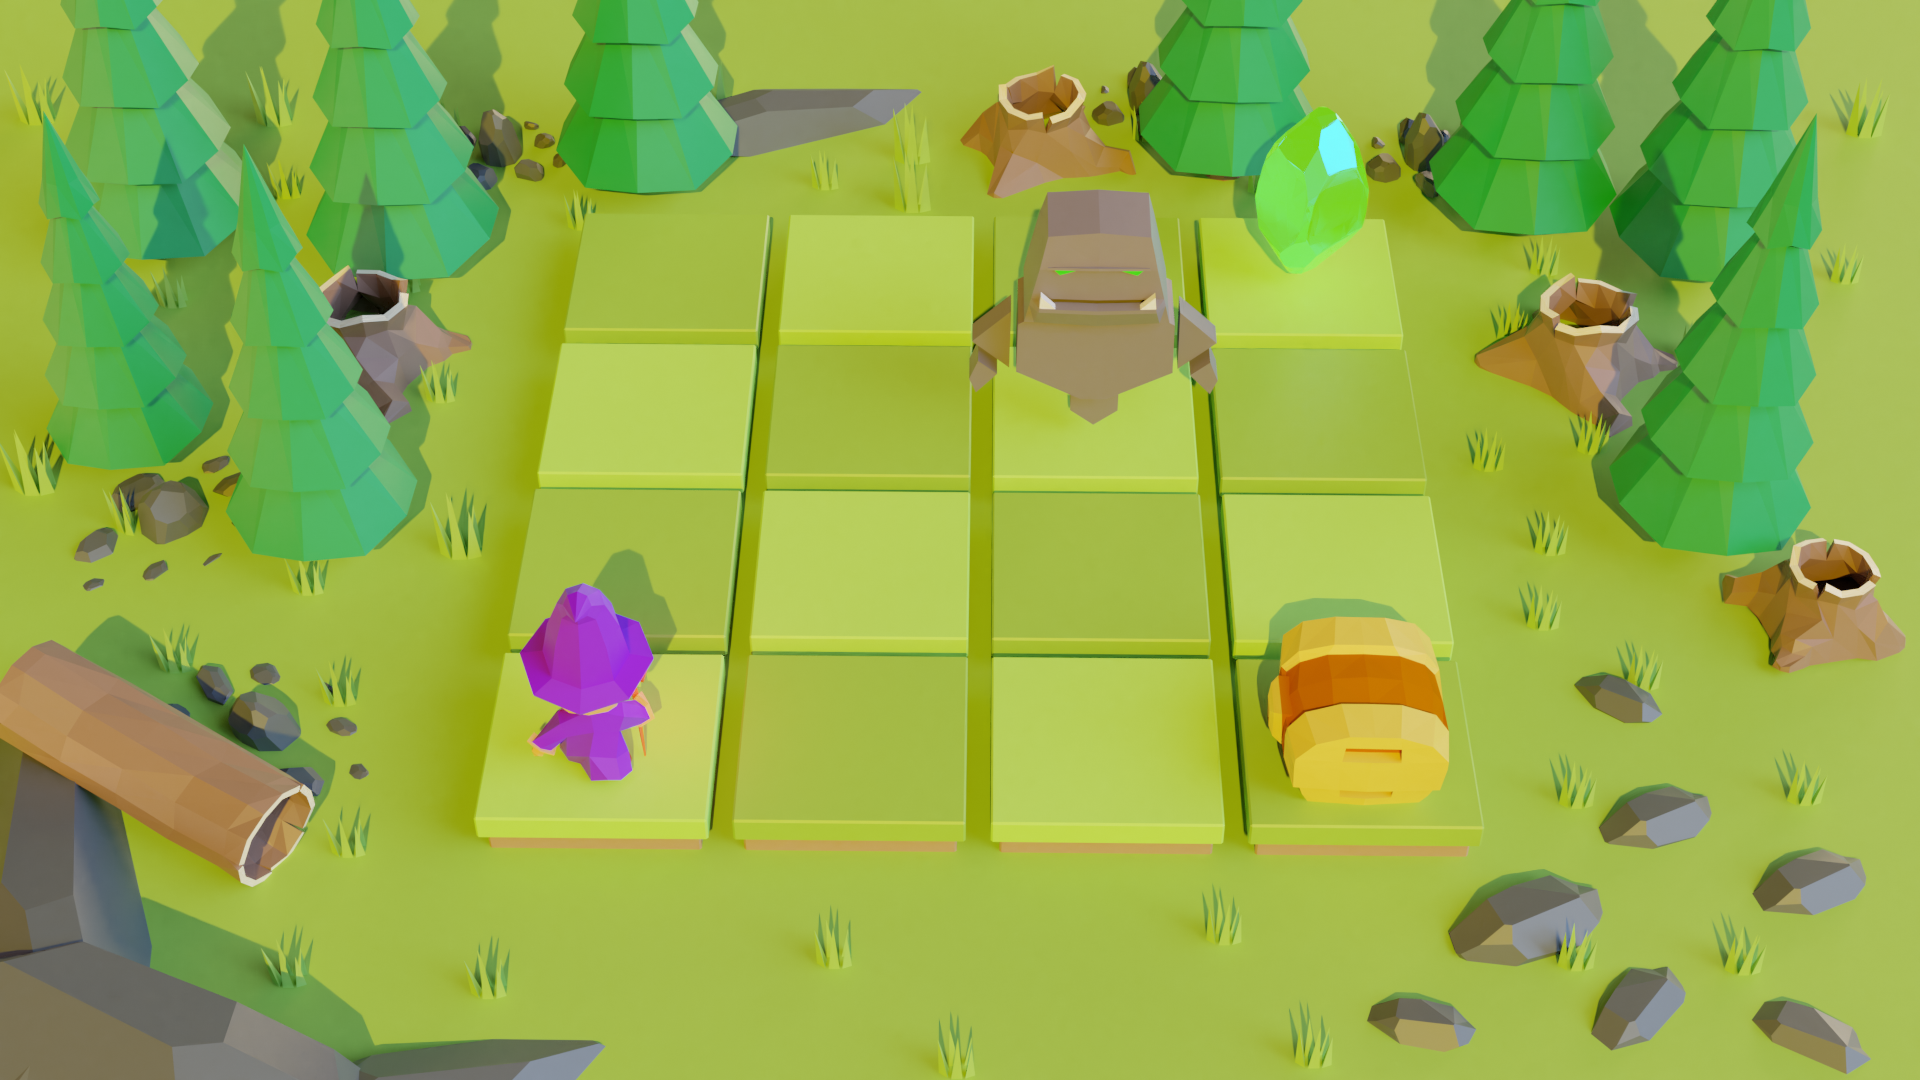
\includegraphics[width=0.6\textwidth]{img/model-levelu.png}
    \caption{Model úrovně.}
    \label{fig:model-levelu}
\end{figure}